% Chapter Template

\chapter{Context, Objectives and Contributions} % Main chapter title

\label{ChapterIntroduction}

%----------------------------------------------------------------------------------------
%	SECTION 1
%----------------------------------------------------------------------------------------

\section{Introduction to Cryptography}
The terms \emph{Cryptography}, from the Greek \emph{krypt\`os} (secret) and \emph{graphein} (writing), and \emph{Cryptanalysis}, denote two branches of a science named \emph{Cryptology}, or \emph{science of the secret}. Cryptography initially refers to the art of \emph{encrypting} messages, which means writing meaningful messages in such a way to appear nonsense to anyone unaware of the encryption process. The readable message is referred to as \emph{plaintext}, while the unintelligible output of the encryption is referred to as \emph{ciphertext}. In general, cryptography aims to construct protocols to secure communication, while cryptanalysis studies the resistance of cryptographic techniques, developing \emph{attacks} to break the cryptosystems' security claims. These two complementary domains evolve in parallel, since the evolution of attack techniques allows conceiving more resistant cryptographic algorithms, and inversely the resistance of such algorithms requires the conception of more sophisticated attacks.\\

The art of cryptography is very ancient, probably as ancient as the language, but only the development of information technology made cryptology take the shape of a proper science, sometimes referred to as \emph{Modern Cryptology}. The last is seen as a branch of different disciplines, such as applied mathematics, computer science, electrical engineering, and communication science. Modern cryptosystems exploit algorithms based on mathematical tools and are implemented as computer programs, or electronic circuits. Their goal is to provide security functionalities for communications that use \emph{insecure channels}, for example the internet. In particular, modern cryptosystems are designed in order to ensure at least one of the four following information security properties:
\begin{itemize}
\item[a.] \emph{confidentiality}: the transmitted message must be readable only by a chosen pool of authorised entities;
\item[b.] \emph{authenticity}: the receiver can verify the identity of the sender of a message;
\item[c.] \emph{non-repudiation}: the sender of a message cannot deny having sent the message afterwards;
\item[d.] \emph{data integrity}: the receiver can be convinced that the message has not been corrupted during the transmission.


\end{itemize} 

Two branches of cryptography may be distinguished: the \emph{symmetric cryptography} and the \emph{asymmetric cryptography}. The first one historically appeared before and is based on the hypothesis that the two communicating entities share a common secret, or secret key; for this reason this is also called \emph{secret key cryptography}. The second one, introduced around 1970, allows any entity to encrypt a message in such a way that only a unique chosen other entity could decrypt it; this is also called \emph{public key cryptography}. \\

A general principle in cryptography, nowadays widely accepted by cryptography researchers, is the one given by Kerckhoff in 19th century: it states that cryptosystems should be secure even if everything about the system, except the key, is public knowledge. Following this principle, today many industrials and governmental agencies exploit, for their security services, cryptosystems based over standardised algorithms. Such algorithms are of public domain, thus have been tested and tried to be broken by a large amount of people, before, during and after the standardisation process. Resistance to many attempts of attacks is actually the strengths of standard algorithms. \\

Low-level cryptographic routines, called \emph{primitives}, are often used as building blocks to construct cryptographic protocols. We provide hereafter a description of a standard primitive, the symmetric AES, whose implementation will be the target of all experiments described in this thesis.

\subsection{Description of AES}
The \emph{Advanced Encryption Standard} (AES) has been standardised in 2001 by the United States governmental agency \emph{National Institute of Standards and Technology} (NIST),\ through the \emph{Federal Information
Processing Standards Publication 197 } (FIPS PUB 197) \cite{nist197}. It is a \emph{block cipher}, meaning that the encryption and decryption of the AES are functions that take as input a string (respectively the plaintext or the ciphertext) of fixed length over the binary alphabet. Indeed, the AES operates on blocks of 128 bits.\footnote{When a block cipher is used to encrypt a plaintext of different size, the plaintext is chunked into blocks of the appropriate one, and each block is encrypted accordingly to a so-called \emph{mode of operation}.} There exist three versions of AES, characterized by the size of the used key: 128, 192 or 256 bits. The encryption is done by rounds. The number of executed rounds depends on the key size (10 rounds for 128 bits, 12 for 192 and 14 pour 256). The basic processing unit in AES algorithm is a byte. For AES internal operations, bytes are arranged on a two-dimensional array called the \emph{state}, denoted $s$. Such a state has 4 rows and 4 columns, thus contains 16 bytes. The byte lying at the $i$-th row, $j$-th column of $s$ will be denoted by $s_{i,j}$ for $i,j\in\{0,1,2,3\}$. The 16 input bytes and the 16 output bytes are indexed column-wise as shown in Fig.~\ref{fig:AES_state}. Each element $s_{i,j}$ of the state is mathematically seen as an element of the \emph{Rjindael finite field}, defined as $GF(2^8) = \mathbb{Z}/{2\mathbb{Z}[X]}/P(X)$ where $P(X) = X^8 + X^4 + X^3 + X + 1$. Five functions are performed during the AES, named KeySchedule, AddRoundKey, SubBytes, ShiftRows and MixColumns. At high level the AES algorithm is described hereafter:
\begin{itemize}
\item[]\textbf{Key Expansion:}  derivation of round keys from secret key through the KeySchedule function
\item[]\textbf{Round 0:}  
\begin{itemize}
\item[] AddRoundKey
\end{itemize}
\item[] \textbf{Rounds 1 to penultimate:}
\begin{itemize}
\item[] SubBytes
\item[] ShiftRows
\item[] MixColumns
\item[] AddRoundKey
\end{itemize}
\item[] \textbf{Last Round:}
\begin{itemize}
\item[] SubBytes
\item[] ShiftRows
\item[] AddRoundKey
\end{itemize}
\end{itemize}

\begin{figure}
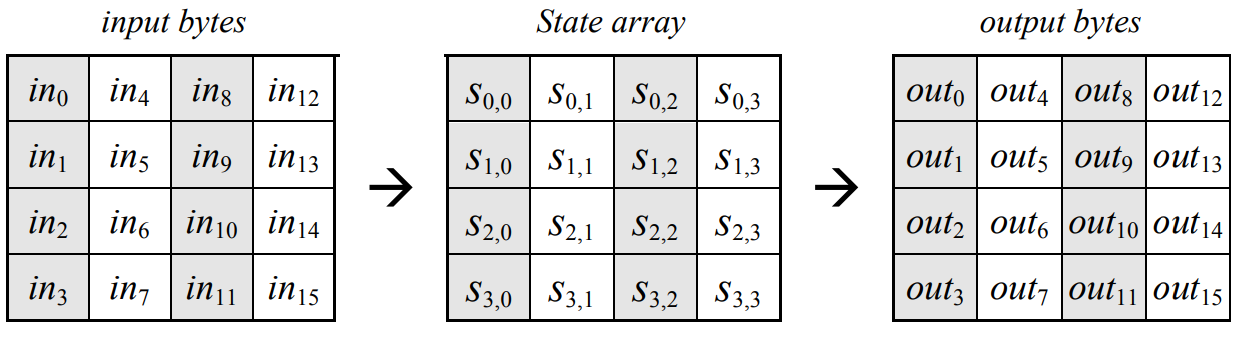
\includegraphics[width = \textwidth]{../Figures/FISP_AES/state.png} 
\caption[State array input and output.]{State array input and output. Source: \cite{nist197}.}\label{fig:AES_state}
\end{figure}

A description of the five functions is provided hereafter.


\subsubsection*{AddRoundKey} Each byte of the state is combined with the corresponding byte of the round key \via an addition over the Rjindael field $GF(2^8)$, \ie a bitwise exclusive OR (\emph{XOR}) operation $\oplus$.
\subsubsection*{SubBytes}
\begin{figure}
\centering
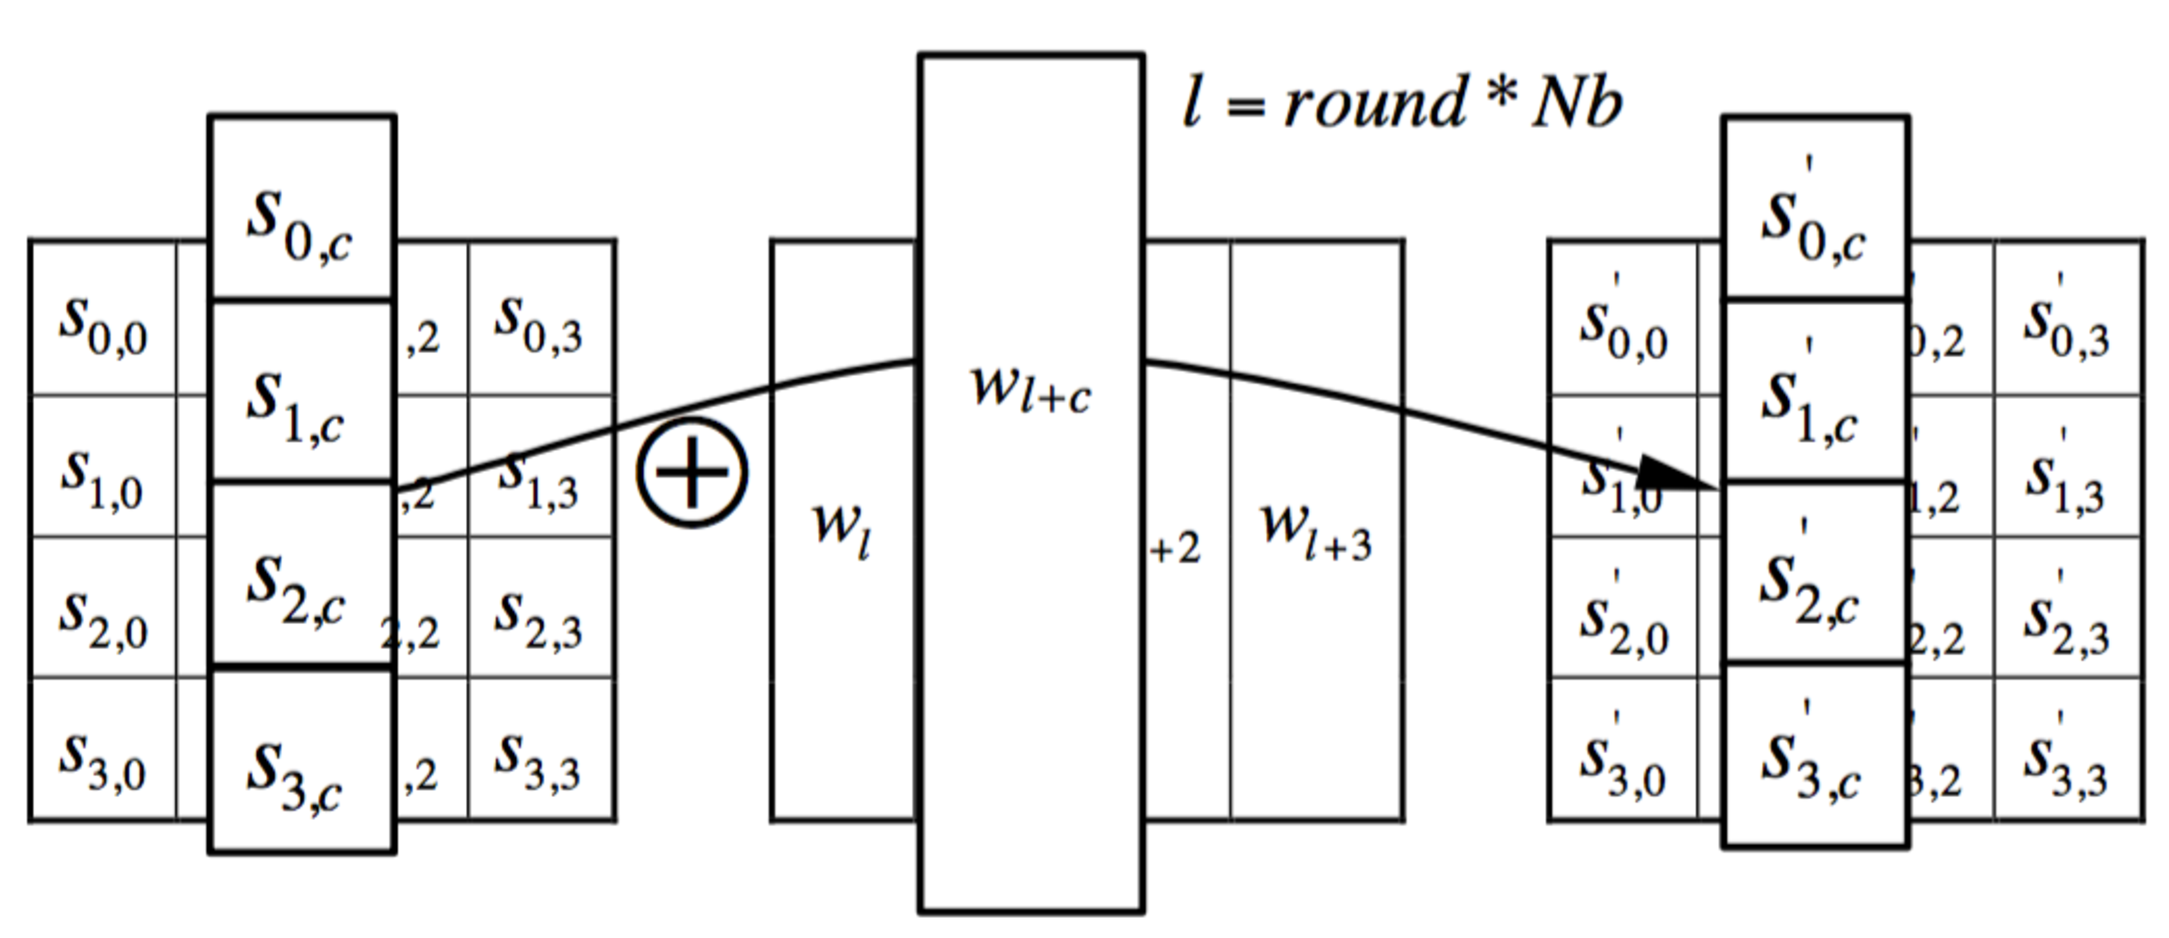
\includegraphics[width = .60\textwidth]{../Figures/FISP_AES/add_round_key.pdf} 
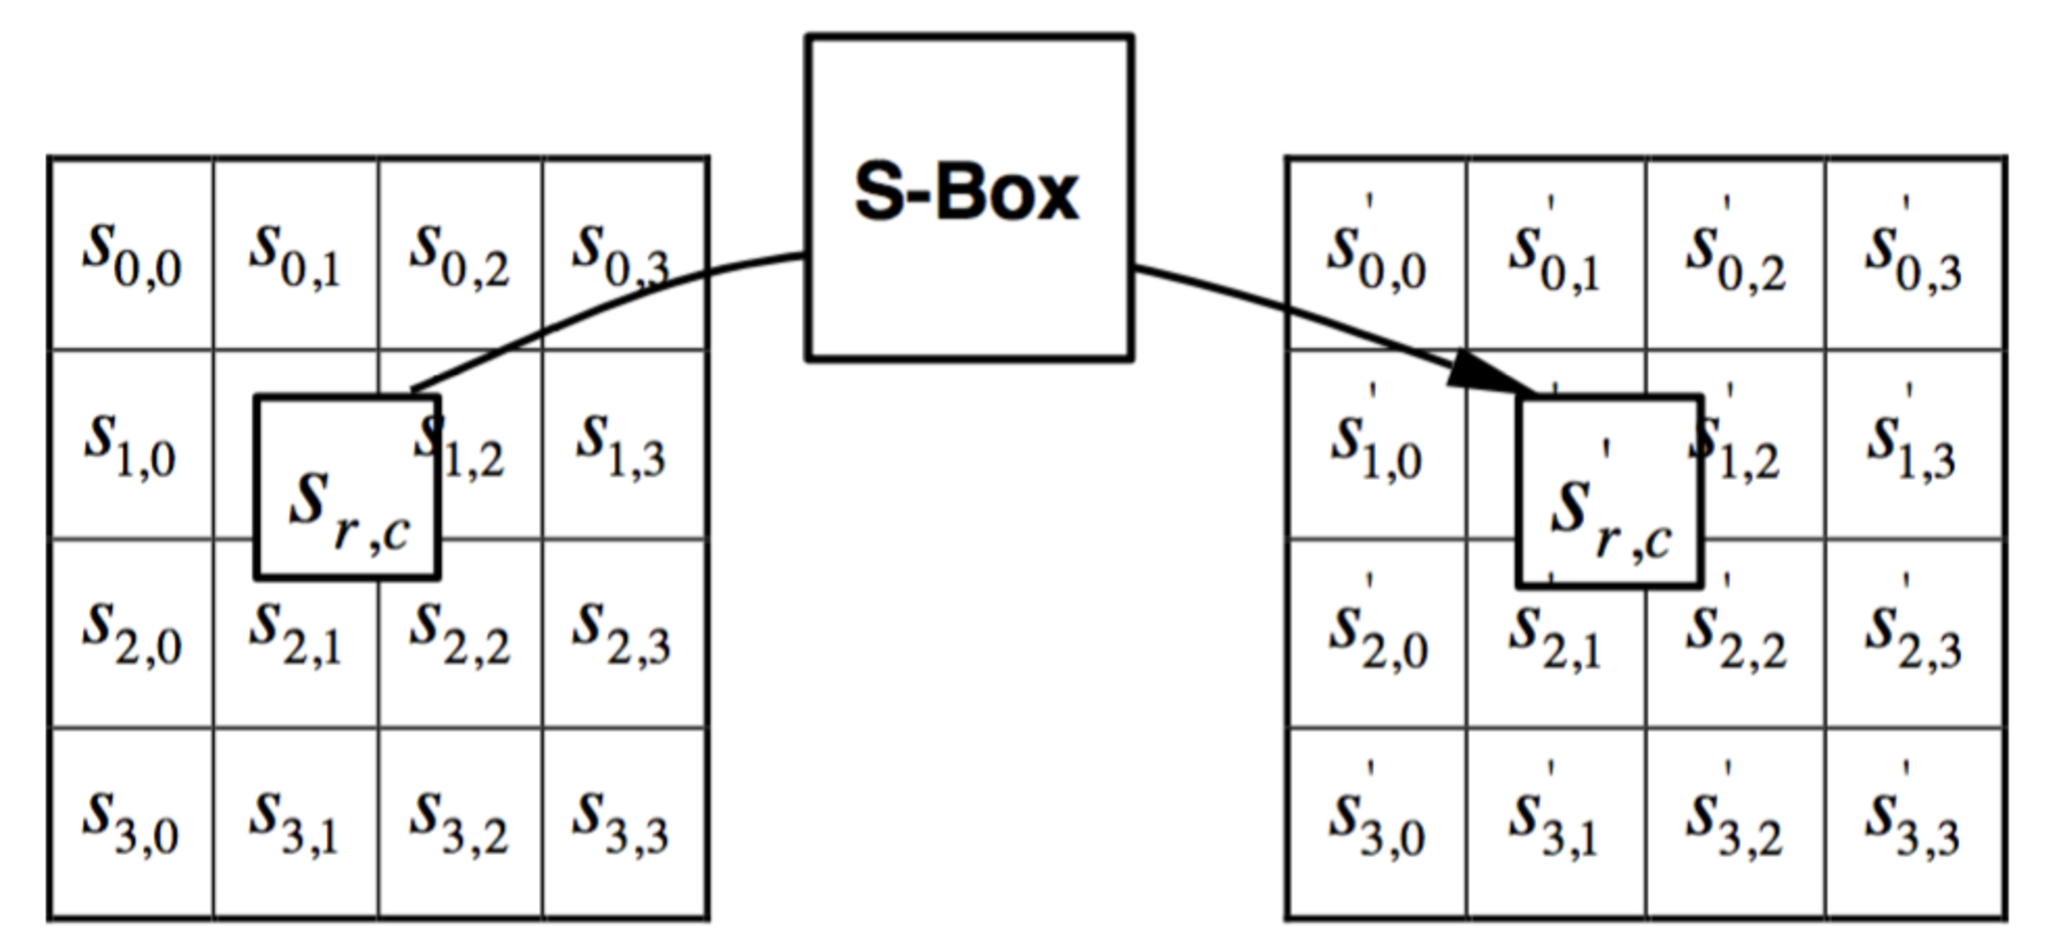
\includegraphics[width = .45\textwidth]{../Figures/FISP_AES/sbox.pdf} 
\caption[AddRoundKey and SubBytes.]{AddRoundKey (top) and SubBytes (bottom) operate over the state byte by byte, independently. Source: \cite{nist197}.}\label{fig:AES_sbox}
\end{figure}
The SubBytes transformation is a non-linear byte invertible substitution that operates independently on each byte of the State using a substitution table (called $\Sbox$). The SubBytes is composed of the following two functions:
\begin{itemize}
\item the inversion in $GF(2^8)$ where the element $\{00\}$ is mapped to itself
\item the affine transformation which maps each byte $b_i$ to:
\begin{equation}
b_i \oplus b_{(i+4)\mbox{mod }8} \oplus b_{(i+5)\mbox{mod }8} \oplus b_{(i+6)\mbox{mod }8} \oplus b_{(i+7)\mbox{mod }8} \oplus c_i \mbox{ ,}
\end{equation}
 where $c_i$ is the $i^\text{th}$ bit of $\{63\}  = (01100011)_2$.
\end{itemize}  
\subsubsection*{ShiftRows}
The bytes in the last second, third and fourth rows of the State are cyclically shifted over 1, 2, and 3 byte(s) respectively.
\subsubsection*{MixColumns}
Each column of the State is treated as a four-term polynomial. They are considered as polynomials over the Rjindael field $GF(2^8)$ and multiplied modulo $X^4 +1$ with a fixed polynomial $a(X) = \{03\}X^3 +\{01\}X^2 + \{01\}X + \{02\}$.

\begin{figure}
\centering
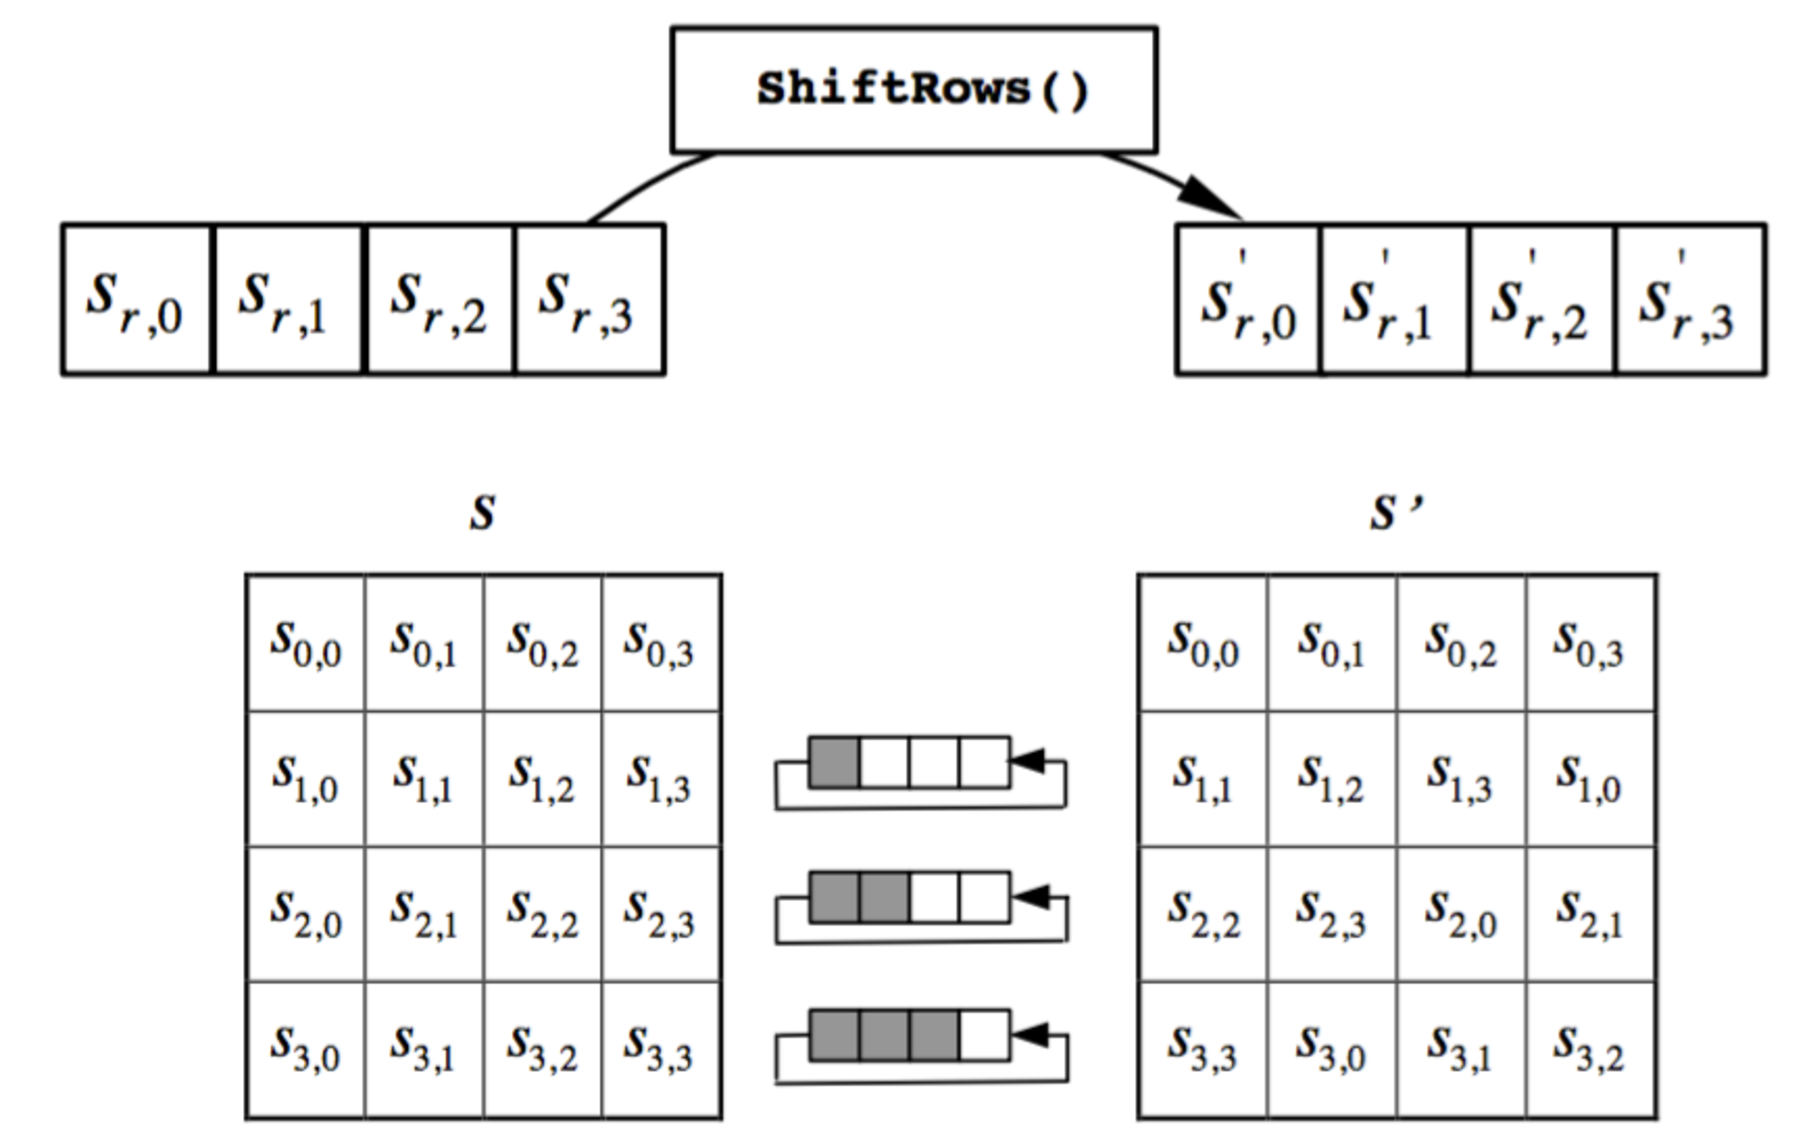
\includegraphics[width = .45\textwidth]{../Figures/FISP_AES/shift_rows.pdf} 
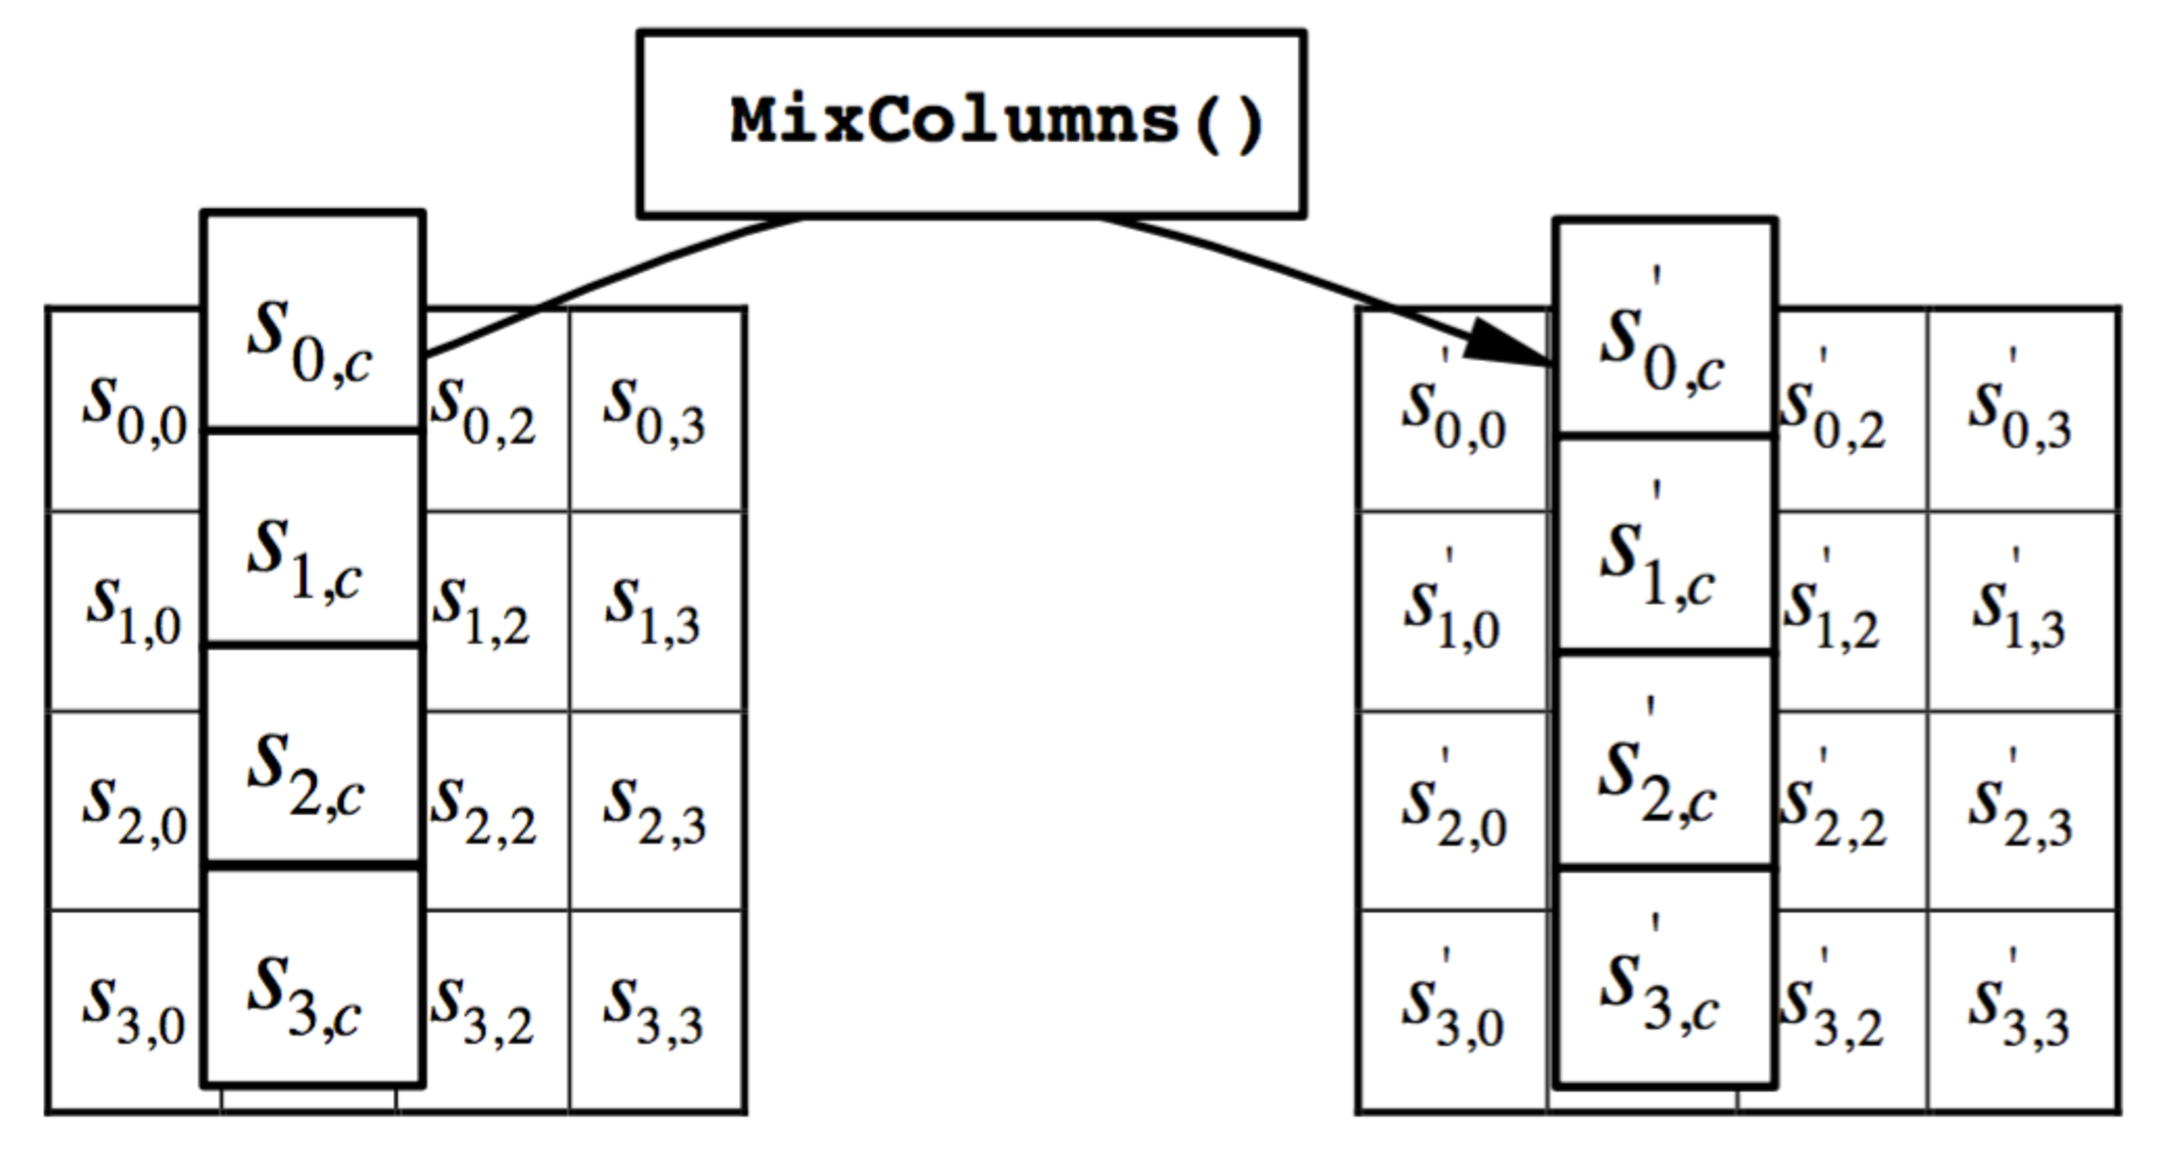
\includegraphics[width = .45\textwidth]{../Figures/FISP_AES/mix_columns.pdf} 
\caption[ShiftRows and MixColumns.]{ShiftRows operates over the State rows. MixColumns operates over the State columns. Source: \cite{nist197}.}\label{fig:AES_sr_mc}
\end{figure}


\subsubsection*{KeySchedule}
To lighten notations, the KeySchedule is described for the 128-bits cipher, which allows to fix many parameters to the value 4. For the 192-bits and 256-bits such parameters have to be fixed respectively to 6 and 8. The key round of the initial round of AES coincides with the secret encryption key $\boldsymbol{K} = (k_{0,0},k_{0,1},\dots,k_{0,3}, k_{1,0},\dots,k_{1,3},\dots,k_{3,3})$. The $i$-th round key is given by 
\begin{equation*}
\boldsymbol{K_i} = (k_{4i,0},k_{4i,1},\dots,k_{4i,3}, k_{4i+1,0},\dots,k_{4i+1,3},\dots,k_{4i+3,3}),
\end{equation*}
where $k_{4i+a,b}$ is calculated, for $i>0$,  $a\in\{0,\dots 3\} $ and $ b\in\{0,\dots,3\}$, as follows: 
\begin{equation*}
\begin{cases}
k_{4i + a,b} = k_{4i +a-4,b}\oplus k_{4i +a-1,b} & \mbox{if } a \neq 0 \\
k_{4i + a,b} = k_{4i +a-4,b}\oplus \Sbox(k_{4i +a-1,(b+1) \mbox{mod } 4}) \oplus \mathrm{Rcon}(a) & \mbox{if } a = 0 \mbox{ and } b=0\\
k_{4i + a,b} = k_{4i+a-4,b}\oplus \Sbox(k_{4i+a-1,(b+1) \mbox{mod } 4})  & \mbox{if } a =0 \mbox{ and } b\neq 0 \mbox{ ,} 
\end{cases}
\end{equation*}

where $Rcon(a) = \{02\}^{a-1}$ in the Rjindael finite field,\footnote{where $\{02\}=(00000010)_2$ is represented by the polynomial $x$} and $\Sbox$ is the substitution table used for the SubBytes transformation.

%\subsection{Description of RSA}
%The RSA cryptosystem, proposed in 1978 by Rivest, Shamir and Adleman \cite{rivest1978method}, represents the first practical realization of the use of trapdoor functions to provide asymmetric cryptography (a concept proposed two years earlier by Diffie, Helman and Merkle \cite{diffie1976new}). RSA is one of the most deployed, analysed, challenged, and discussed cryptosystems of all times, the seminal paper \cite{rivest1978method} counting today $18,950$ citations.\footnote{From Google Scholar, visited on January 2018.}\\
%
%Hereafter a simplified description of the RSA algorithm is provided.\\
%Let $N = p \times q$ be the product of two large primes of about the same size. Then we can compute two values $e,d$ such that $e$ and $\varphi(N)$ are co-prime and $d = e^{-1} (\mbox{mod } \varphi(N))$, where $\varphi(N) = (p-1)\times(q-1)$ is the Euler's totient function of $N$, corresponding to the size of the multiplicative group $	\mathbb{Z}^\star_N$. The pair $(N,e)$ is the public key, and $d$ is the private one. Let $M \in	\mathbb{Z}^\star_N$ be a message. The encryption of $M$ is defined as the operation $C = M^e (\mbox{mod } N)$. The ciphertext $C$ can then be decrypted by computing $C^d (\mbox{mod } N)$. The fact that the two transformations are mutually inverse is a consequence of Euler's totient theorem. As $e$ denotes the public exponent, everyone is allowed to encrypt a message addressed to the owner of the private key $d$, who is the only entity able to retrieve the original message. The security of such a cryptosystem is based on the big integers factorization problem.\\
%Using the same operations, RSA can easily be used for signature applications as well: in this case the operation $S = M^d (\mbox{mod } N)$ can be used by the owner of the secret key $d$ to sign the message $M$. Everyone provided with the message $M$ and the signature $S$ is then allowed to verify the signature, using the public key $(N,e)$ and the inverse operation $M = S^e (\mbox{mod } N)$.


%----------------------------------------------------------------------------------------
%	SECTION 2
%----------------------------------------------------------------------------------------
\section{Secure Components}

As we have seen in the previous section, modern cryptography proposes solutions to secure communications that ask for electronic computations and repose their security over some secret keys. Keys are represented as long bit strings, very hard to be memorised by users. Thus, keys need to be stored in a secure medium, and never delivered in clear over insecure channels. Smart cards (or smartcards) were historically conceived as a practical solution to such a key storage issue: they consist in small devices a user can easily carry around with, which not only store secret keys, but also are able to internally perform cryptographic operations, in such a way that they can be involved in secure communication protocols, that do not require the delivering of the secret keys. The registrations of a first patent describing memory cards by Roland Moreno in 1974 \cite{moreno}, and of a second one describing cards equipped with microcontrollers by Michel Ugon in 1977 \cite{ugon} are often referred to in order to date the smart card invention, finally produced for the first time in 1979. Smart cards are pocket-sized plastic-made cards equipped with a secure component, which is typically an integrated circuit containing some computational units and some memories.\\

Today, about 40 years after its invention, they still have a huge diffusion, both in terms of applicative domains and in terms of quantity of exemplars. Indeed, they serve as credit or ATM cards, healthy cards, ID cards, public transport payment cards, fuel cards, identification and access badges, authorization cards for pay television, etc. Slightly changing the card support, we find other applications of the same kind of integrated circuits, for example the  mobile phone SIMs (\emph{Subscriber Identity Module}) and the electronic passports. In terms of quantity, a marketing research \cite{ABI} found out that in 2014 8.8 billion smart cards have been sold, \emph{i.e.} the same order of magnitude of the global population. \\

In addition to smart cards, the recent growing and variation of security needs lead to the development and specification of other kinds of secure solutions, for example the \emph{Trusted Platform Module} 
(TPM), which is a secure element providing cryptographic functionalities to a motherboard, or completely different solutions based on software layers, that are today in great expansions. An example is provided by the \emph{Trusted Execution Environment} (TEE), which is a software environment of the main processor of a smartphone or tablet, designed to assure resistance to software menaces. 

\subsection{Embedded Cryptography Vulnerabilities}\label{sec:vulnerabilities}
\subsubsection{Side-Channel Attacks}\label{sec:SCAintro}
Until the middle of the nineties, the security of embedded cryptosystems was considered, in the public domain, as equivalent to the mathematical security of the embedded cryptographic algorithm. In classical cryptanalysis, an attacker usually has the knowledge of the algorithm (in accordance to Kerckhoff's principle) and of some inputs and/or outputs. Starting from these data, his goal is to retrieve the secret key. This attack model considers the algorithm computation as a black box, in the sense that no internal variable can be observed during execution, only inputs and/or outputs. With his seminal paper about Side-Channel Analysis in 1996, Paul Kocher showed that such a black-box model fails once the algorithm is implemented over a physical component \cite{kocher1996timing}: an attacker can indeed inspect its component during the execution of the cryptographic algorithm, monitor some physical quantities (\eg the execution time \cite{kocher1996timing} or the instantaneous power consumption \cite{kocher1999differential}) and deduct information about internal variables of the algorithm. Depending on the attacked algorithm, making inference over some well chosen internal variables (the so-called \emph{sensitive variables} of the algorithm) is sufficient to retrieve the secret key. After these first works, it was shown that other observable physical quantities contained \emph{leakages} on sensitive information; for example the electromagnetic radiation emanating from the device \cite{gandolfi2001electromagnetic,quisquater2001electromagnetic} and the acoustic emanations \cite{genkin2014rsa}. Moreover, if until few years ago it was thought that only small devices, equipped with slow microprocessors and with small-sized architecture, such as smart cards, were vulnerable to this kind of Side-Channel Attacks, the last cited recent work about acoustic emanations, together with other works exploiting electromagnetic fluctuations, pointed out that much faster and bigger devices, \emph{i.e.} laptops and desktop computers, are vulnerable as well \cite{genkin2015stealing,genkin2015get,genkin2016ecdh}.

\subsubsection{A Classification of the Attacks against Secure Components}\label{sec:classification_attacks}
\begin{table}[]
\centering
\caption{Classification of Harware Attacks}
\label{fig:classification_attacks}
\begin{tabular}{l|l|l|}
\cline{2-3}
                                    & Passive & Active \\ \hline
\multicolumn{1}{|l|}{Invasive}      &         &        \\ \hline
\multicolumn{1}{|l|}{Semi-Invasive} & (SCAs)  & (FAs)  \\ \hline
\multicolumn{1}{|l|}{Non-Invasive}  & SCAs    & FAs    \\ \hline
\end{tabular}
\end{table}

The Side-Channel Attacks outlined in previous paragraph, and which are the main concern of this thesis,  belong to a much bigger family of hardware attacks that can be performed to break cryptographic devices' security claims. A classification for hardware attacks is briefly outlined in Tab.~\ref{fig:classification_attacks}. They are commonly classified on the base of two criteria: on one hand we can distinguish passive and active attacks, on the other hand we can distinguish invasive, semi-invasive and non-invasive attacks. 
\begin{itemize}
\item[] \textbf{Passive attacks:} in passive attack, the device run respecting its specifications. The attacker observes its behaviour without provoking any alteration;
\item[] \textbf{Active attacks:}  in active attacks a special manipulation is performed in order to corrupt the normal behaviour of the device. 
\end{itemize}


\begin{itemize}
\item[] \textbf{Invasive attacks}: in invasive attacks, the device is unpackaged and inspected at the level of the component technology. The circuit can be modified/broken, signals can be accessed \via a probing station, etc. There is no limits to the manipulations an attacker can do to the component;
\item[] \textbf{Semi-invasive attacks}: as in invasive attacks the device is unpackaged, but in contrast to them, no direct electrical contact to the chip is done;
\item[] \textbf{Non-invasive attacks}: in non-invasive attacks the device is not modified and only accessible interfaces are exploited. 

\end{itemize}

In the literature, the term Side-Channel Attacks (SCAs)\footnote{Commonly, the acronym SCA stands for \textquotedbl Side-Channel Analysis\textquotedbl. Nevertheless, in this thesis it will stand for \textquotedbl Side-Channel Attacks\textquotedbl.} commonly refers to the passive non-invasive attacks. Nevertheless, the techniques proposed under the name of SCAs, that always require the acquisition of some signals, might also include attacks where the device is unpacked, in order to improve the signal amplitude. In this sense, SCAs belong to the semi-invasive group of attacks as well. Similarly, active non-invasive attacks are often referred to as \emph{Fault Injection Attacks}, that might also be run in a semi-invasive way.\\

Beyond hardware attacks, there exists a second class of attacks that menaces the security of cryptographic devices: the software attacks. In contrast with hardware attacks, software attacks exploit vulnerabilities that are not related to the physical implementation of the cryptographic functionalities of the device: they are not based on hypotheses about the material execution of the cryptographic algorithms, but exploit vulnerabilities of the software interfaces. A typical example of software attack consists in charging malware code into the device, enabling access to data and instructions contained in memories (RAM or ROM), in order to retrieve, modify or destroy information they hold. In last years, together with the growing complexity of secure devices, attacks become more and more sophisticated and the boundary between hardware and software attack is more and more blurred. Moreover combined software/hardware attacks are being developed,\eg \cite{bouffard2011combined}.



\subsection{Certification of a Secure Hardware - The Common Criteria}
\begin{figure}
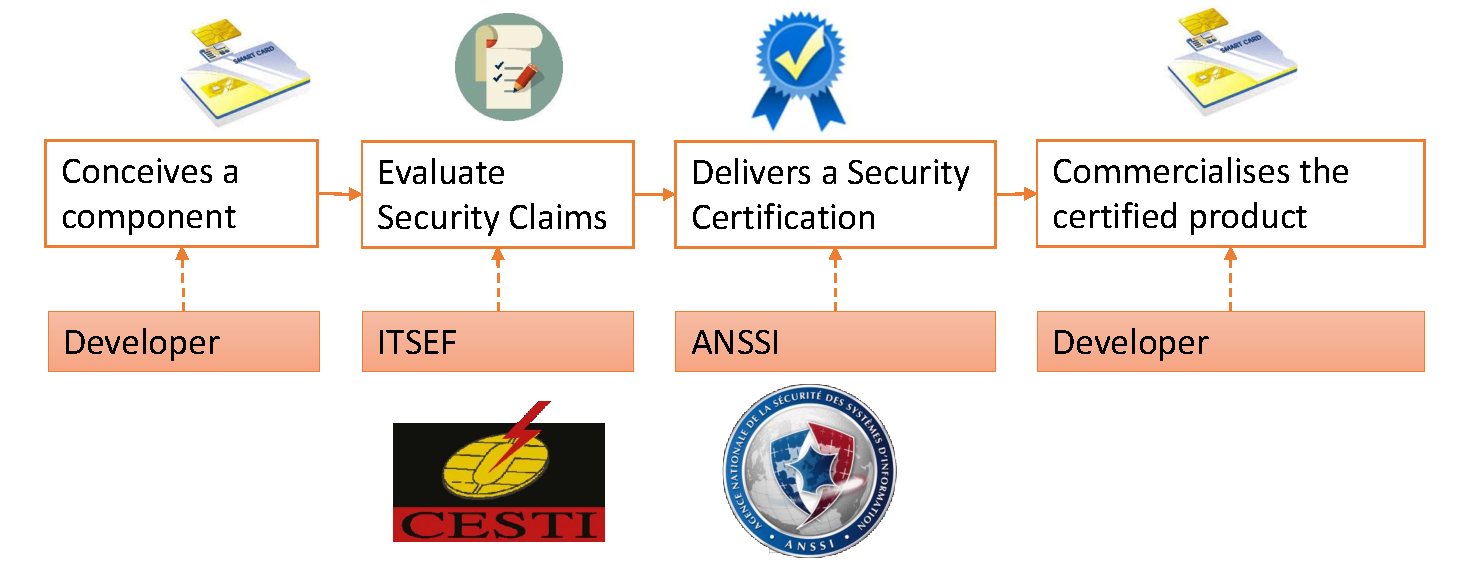
\includegraphics[width=\textwidth]{../Figures/ITSEF_ANSSI2.pdf} 
\caption{The actors of French Certification Scheme}
\end{figure}
In previous paragraphs we have evoked the great diffusion of the cryptographic devices and the existence of a wide range of attacks exploiting vulnerabilities coming from the way cryptography is embedded. These two factors imply a great risk related to the production and commercialisation of such devices, and justify the importance and necessity to ensure reliability on their security claims. This necessity lead to the arise of several guidelines and standards for their evaluation. The international standard ISO/IEC 15408, also known as \emph{Common Criteria for Information Technology Security Evaluation} (abbreviated as \emph{Common Criteria} or simply \emph{CC}) represents one of the strongest efforts in standardisation, unifying in 1999 three previously existing standards:
\begin{itemize}
\item the \emph{Trusted Computer System Evaluation Criteria} (TCSEC - United States - 1983)
\item the \emph{Information Technology Security Evaluation Criteria} (ITSEC - France,Germany, Netherlands, United Kingdom - 1990)
\item the \emph{Canadian Trusted Computer Product Evaluation Criteria} (CTCPEC - Canada - 1993).
\end{itemize}

\subsubsection{The actors} The CC define four actors of the evaluation process of a secure component:
\begin{itemize}
\item \textbf{The Developer}, who conceives a product and wishes to sell it as a certified secure product. He sends a request for evaluation to the certification body and, once the request is accepted, he contacts an evaluation laboratory;
\item \textbf{The ITSEF} is the \emph{IT Security Evaluation Facility}; in France it is named \emph{Centre d'Evaluation de la Securit\'e des Technologies de l'Information} (CESTI). It is an evaluation laboratory, in possession of a certification body agreement, which performs the security tests to assess the resilience of the product;
\item \textbf{The Certification Body} is often a governmental organism, the \emph{Agence National de la Securit\'e des Syst\`emes d'Information} (ANSSI) in France, or the \emph{Bundesamt f\"ur Sicherheit in der Informationstechnik} (BSI) in Germany, for example. It ensures the quality of the evaluation and delivers a certificate to the developer;
\item \textbf{The end user}, who buys the product and follows its security guidelines.
\end{itemize} 

\subsubsection{The Target of Evaluation and the security objectives} 
To start the certification process, the developer compiles a document called \emph{Security Target} (ST). Such a document begins specifying the (part of the) device subjected to evaluation, the so-called \emph{Target of Evaluation} (TOE), then lists its \emph{Security Functional Requirements} (SFR), choosing among those proposed by the CC. In practice, and to ease the redaction of the ST, the choice of the SFRs is not open, but guided by the typology of the component. In particular, the CC propose a catalogue of \emph{Protection Profiles}, associated with the required SFRs. For example \textquotedbl smartcard\textquotedbl \ or \textquotedbl TEE \textquotedbl \  designate some precise Protection Profiles. They differ in various aspect, and their main difference until now is that TEE are not required to be resistant to hardware attacks, but only software ones. the recent alerts about combined software/hardware attacks developed in last years, may lead to an extension of the solely software vulnerability analysis towards a larger requirement.

\subsubsection{Evaluation Assurance Level and Security Assurance Requirements}
\begin{table}[]
\centering
\caption{Evaluation Assurance Levels}
\label{tab:EAL}
\begin{tabular}{cc}
\toprule 
EAL  & Description                                \\
\midrule
EAL1 & Functionally tested                        \\
EAL2 & Structurally tested                        \\
EAL3 & Methodically tested and checked            \\
EAL4 & Methodically designed, tested and reviewed \\
EAL5 & Semi-formally designed and tested          \\
EAL6 & Semi-formally verified design and tested   \\
EAL7 & Formally verified design and tested      \\
\bottomrule
\end{tabular}
\end{table}

In CC seven  \emph{Evaluation Assurance Level} (EAL) are defined. They determine the quantity and complexity of the tasks the evaluator has to effectuate, thus specifying the insurance strength. The EAL are defined in insurance increasing order, so that the EAL1 has the lowest verification exigences while EAL7 has the highest ones. In Table~\ref{tab:EAL} the objectives given by the CC for each EAL are resumed.\\

During the process of evaluation, the SFRs of the TOE have to be verified according to the claimed EAL. To this end, the evaluation is  divided into six classes of \emph{Security Assurance Requirement} (SAR). Five of this classes are the so-called \emph{conformity} classes, and one is the \emph{vulnerability assessment} class. Each class is sub-divided in several \emph{families} (excepted the vulnerability assessment class, which only contains one family), and the evaluators are charged to check each requirement corresponding to these families. The Table~\ref{tab:SAR} resumes the SAR classes and their families. For each family a grade is assigned following precise specifications detailed in CC, and the obtention of a certain EAL depends on the grades obtained for each family, as reported in Table~\ref{tab:components}. An EAL can also be \emph{augmented}, meaning that the product achieves all the required SAR grades to obtain a certain EAL and some upper grades for certain families. For example, smart cards are usually protected at level EAL4$+$AVA\_VAN5$+$ALC\_DVS2, and chips for e-passport application are usually protected at level EAL5$+$AVA\_VAN5$+$ALC\_DVS2. In case of banking smart cards, the card also needs to respect the EMVco norms, being EMVco a consortium of six companies (Visa, MasterCard, JCB, American Express, China UnionPay, and Discover) that manages private certification schemes for banking cards, payment terminal and automated teller machines. 


\begin{table}[]
\centering
\caption{Security Assurance Requirements}
\label{tab:SAR}
\begin{tabular}{ccc}
\toprule
Class                               & Family   & Description                           \\
\midrule
\multirow{6}{*}{Development}        & ADV\_ARC & Security architecture                 \\
                                    & ADV\_FSP & Functional specification              \\
                                    & ADV\_IMP & Implementation representation         \\
                                    & ADV\_INT & TOE Security Functions internals      \\
                                    & ADV\_SPM & Security policy modelling             \\
                                    & ADV\_TDS & TOE design                            \\
                                    \midrule
\multirow{2}{*}{Guidance Documents} & AGD\_OPE & Operational user guidance             \\
                                    & AGD\_PRE & Preparative procedures                \\
                                    \midrule
\multirow{7}{*}{Life-cycle support} & ALC\_CMC & Configuration Management capabilities \\
                                    & ALC\_CMS & Configuration Management scope        \\
                                    & ALC\_DEL & Delivery                              \\
                                    & ALC\_DVS & Development security                  \\
                                    & ALC\_FLR & Flaw remediation                      \\
                                    & ALC\_LCD & Life-cycle definition                 \\
                                    & ALC\_TAT & Tools and techniques                  \\
                                    \midrule
\multirow{7}{*}{ST evaluation}      & ASE\_CCL & Conformance claims                    \\
                                    & ASE\_ECD & Extended components definition        \\
                                    & ASE\_INT & ST introduction                       \\
                                    & ASE\_OBJ & Security objectives                   \\
                                    & ASE\_REQ & Security requirements                 \\
                                    & ASE\_SPD & Security problem definition           \\
                                    & ASE\_TSS & TOE summary specification             \\
                                    \midrule
\multirow{4}{*}{Tests}              & ATE\_COV & Coverage                              \\
                                    & ATE\_DPT & Depth                                 \\
                                    & ATE\_FUN & Functional tests                      \\
                                    & ATE\_IND & Independent testing                   \\
                                    \midrule
Vulnerability assessment            & AVA\_VAN & Vulnerability analysis   \\
\bottomrule
            
\end{tabular}
\end{table}



\begin{table}[]
\centering
\caption{Required grades for the obtention of each EAL.}
\label{tab:components}
\begin{tabular}{|c|c|c|c|c|c|c|c|}
\hline
\multirow{2}{*}{Family} & \multicolumn{7}{c|}{Assurance Components by EAL} \\ \cline{2-8} 
                        & EAL1  & EAL2  & EAL3 & EAL4 & EAL5 & EAL6 & EAL7 \\
                        \midrule
ADV\_ARC                &       & 1     & 1    & 1    & 1    & 1    & 1    \\ 
ADV\_FSP                & 1     & 2     & 3    & 4    & 5    & 5    & 6    \\ 
ADV\_IMP                &       &       &      & 1    & 1    & 2    & 2    \\ 
ADV\_INT                &       &       &      &      & 2    & 3    & 3    \\ 
ADV\_SPM                &       &       &      &      &      & 1    & 1    \\ 
ADV\_TDS                &       & 1     & 2    & 3    & 4    & 5    & 6    \\
\midrule
AGD\_OPE                & 1     & 1     & 1    & 1    & 1    & 1    & 1    \\ 
AGD\_PRE                & 1     & 1     & 1    & 1    & 1    & 1    & 1    \\ 
\midrule
ALC\_CMC                & 1     & 2     & 3    & 4    & 4    & 5    & 5    \\ 
ALC\_CMS                & 1     & 2     & 3    & 4    & 5    & 5    & 5    \\ 
ALC\_DEL                &       & 1     & 1    & 1    & 1    & 1    & 1    \\ 
ALC\_DVS                &       &       & 1    & 1    & 1    & 2    & 2    \\ 
ALC\_FLR                &       &       &      &      &      &      &      \\ 
ALC\_LCD                &       &       & 1    & 1    & 1    & 1    & 2    \\ 
ALC\_TAT                &       &       &      & 1    & 2    & 3    & 3    \\ 
\midrule
ASE\_CCL                & 1     & 1     & 1    & 1    & 1    & 1    & 1    \\ 
ASE\_ECD                & 1     & 1     & 1    & 1    & 1    & 1    & 1    \\ 
ASE\_INT                & 1     & 1     & 1    & 1    & 1    & 1    & 1    \\ 
ASE\_OBJ                & 1     & 2     & 2    & 2    & 2    & 2    & 2    \\ 
ASE\_REQ                & 1     & 2     & 2    & 2    & 2    & 2    & 2    \\ 
ASE\_SPD                &       & 1     & 1    & 1    & 1    & 1    & 1    \\ 
ASE\_TSS                & 1     & 1     & 1    & 1    & 1    & 1    & 1    \\ 
\midrule
ATE\_COV                &       & 1     & 2    & 2    & 2    & 3    & 3    \\ 
ATE\_DPT                &       &       & 1    & 1    & 3    & 3    & 4    \\ 
ATE\_FUN                &       & 1     & 1    & 1    & 1    & 2    & 2    \\ 
ATE\_IND                & 1     & 2     & 2    & 2    & 2    & 2    & 3    \\ 
\midrule
AVA\_VAN                & 1     & 2     & 2    & 3    & 4    & 5    & 5    \\ \hline
\end{tabular}
\end{table}

\subsubsection{The AVA\_VAN family and the Attack Potential}
The AVA\_VAN is the solely family of the vulnerability assessment SAR. The goal of such a SAR is to make the connection between the conformity of the TOE, verified \via the analysis of its documentation, and the efficiency of its protections and countermeasures. This is the step of the evaluation in which the actual resilience of the TOE against the \emph{penetration tests} is measured. In this phase the attacks outlined in Sec.~\ref{sec:vulnerabilities} are taken into account, and the so-called \emph{attack potential} of such attacks is stated. The attack potential is a notion appearing in CC whose aim is to reflect the realism of succeeding a certain attack, and thus its realistic dangerousness. Indeed in the context of physical attacks, many possible attack paths require unrealistic conditions, amounts of time and/or money to be actually performed on the field and do not represent in reality a great risk. For example, invasive attacks such as probing attacks which appears in theory the most dangerous ones, ask in general for some very expensive instruments, a huge expertise, much time and many broken samples before succeeding. Their attack potential can thus result not so wondering. For this evaluation phase, the evaluator is in charge to prepare a testing plan. This is a list of the possibly dangerous attack paths, basing on a code analysis, and on the state-of-the-art attacks list in general provided by working groups dedicated to the secure component considered. Once the testing plan is ready, he practically tests each attack. For each succeeded attack he fills a \emph{cotation table} in order to assign a score to the attack, on the basis of several criteria. The goal of the cotation table is to provide a metric enabling to compare very different kinds of attacks. The guidelines for the cotation table are given by the \emph{Common Methodology for Information Technology Security Evaluation} (CEM). \\

In the case of smart cards, the evaluation systematically includes the AVA\_VAN5 grade, thus the testing plan is asked to be as complete as possible. The state-of-the-art of the attacks is periodically upgraded by the \emph{JIL\footnote{Joint Interpretation Library} Hardware Attacks Subgroup} (JHAS), a subgroup of the working committee \emph{Senior Officials Group Information Systems Security} (SOG-IS) which coordinates the standardisation of CC. Moreover, the JHAS produces the \emph{Application of Attack Potential to Smartcards} \cite{JIL} of the JIL, which is an interpretation of the CEM in the special case of smart cards. The cotation table factors specified by the JHAS are detailed in Table~\ref{tab:cot_table}. The evaluation is divided in two parts, an \emph{identification} part, that reflects the difficulty in finding the attack path, and an \emph{exploitation} part, that reflects the difficulty in actually performing the attack. The total score of an attack is the sum of scores assigned to each factor. To obtain the AVA\_VAN5 grade every successful attack tested by the evaluators must have been rated at least 31.\\



\begin{table}[]
\centering
\caption{Factors of the \emph{Attack Potentials for Smartcards}}
\label{tab:cot_table}
\begin{tabular}{ccc}
\toprule
Factors                       & Identification & Exploitation \\
\midrule
\textbf{Elapsed Time}         &                &              \\
\textless one hour            & 0              & 0            \\
\textless one day             & 1              & 3            \\
\textless one week            & 2              & 4            \\
\textless one month           & 3              & 6            \\
\textgreater one month        & 5              & 8            \\
\midrule
\textbf{Expertise}            &                &              \\
Layman                        & 0              & 0            \\
Proficient                    & 2              & 2            \\
Expert                        & 5              & 4            \\
Multiple Expert               & 7              & 6            \\
\midrule
\textbf{Knowledge of the TOE} &                &              \\
Public                        & 0              & 0            \\
Restricted                    & 2              & 2            \\
Sensitive                     & 4              & 3            \\
Critical                      & 6              & 5            \\
Very critical hardware design & 9              & NA           \\
\midrule
\textbf{Access to TOE}        &                &              \\
\textless 10 samples          & 0              & 0            \\
\textless 30 samples          & 1              & 2            \\
\textless 100 samples         & 2              & 4            \\
\textgreater 100 samples      & 3              & 6            \\
\midrule
\textbf{Equipement}           &                &              \\
None                          & 0              & 0            \\
Standard                      & 1              & 2            \\
Specialized                   & 3              & 4            \\
Bespoke                       & 5              & 6            \\
Multiple Bespoke              & 7              & 8            \\
\midrule
\textbf{Open Samples}         &                &              \\
Public                        & 0              & NA           \\
Restricted                    & 2              & NA           \\
Sensitive                     & 4              & NA           \\
Critical                      & 6              & NA    \\	
\bottomrule      
\end{tabular}
\end{table}


\subsubsection{The Evaluation Technical Report}
The evaluation ends with the redaction by the evaluators of an \emph{Evaluation Technical Report} (ETR), which is transmitted to the certification body. The last analyses the ETR and, if the security claims of the TOE are verified, issues a \emph{certificate}. The ETR is kept confidential. Concerning the penetration testing of a certified smart card, the ETR contains all the cotation tables of the succeeded attacks. If the component is certified, it means that the score of those attacks was higher than 31, and such vulnerabilities are kept as \emph{residual vulnerabilities}. The ETR is strictly reviewed annually by the evaluators in charge of the surveillance of the certificate. For the penetration testing, the evaluators are in particular asked each year to verify that the cotation of the attacks presented in the ETR did not drop.

\section{This thesis objectives and contributions}\label{sec:this_thesis_objectives}
Among the factors observable in the cotation table~\ref{tab:cot_table} we find \emph{open samples}, interpretable as \emph{device with known secrets}. Indeed, for an evaluation scope it is sometimes possible for an ITSEF to have access to a device identical to the TOE but where the evaluator can fix or access certain variables, for example some random numbers used by cryptographic algorithm, or load specific software. An evaluator may use this possibility in order to launch executions in which he is aware of the complete execution flow, including operations, manipulated internal variables (internally generated random ones as well) and register accesses. In this way he can understand and characterise the relations between the internal behaviour of the device and the physical observations, before performing a proper attack. \\

In the context of Side-Channel Attacks, when such a characterisation phase is possible, we talk about \emph{profiling attacks}. Due to the favourable condition of this attacks, they are commonly considered the most dangerous ones, allowing a sort of worst-case security analysis. This thesis is mainly focused over such a profiling scenario. Indeed, we will address the problems an evaluator deals with when he is in such a favourable case and he wonders how to optimally exploit such a characterisation phase in order to be able to extract as much information as possible for the acquired signals, in the exploitation phase. One of these issues is the selection of the so-called \emph{Points of Interest} (PoI), strictly linked to the more general problem of dimensionality reduction.

\subsection{The Preliminary Purpose of this Thesis: Research of Points of Interest}\label{sec:foreword}
To perform a Side-Channel Attack, the monitoring of unintentional channels leaking from the attacked device is usually performed through an oscilloscope that samples continuous analog signals and turns them into discrete digitalised sequences. Such sequences are often referred to as \emph{traces}. To allow a deep inspection of the device, the sampling rate of the oscilloscope needs to be high, leading very often to a high dimensionality of such traces. Nevertheless,  it is expected that only a limited number of time samples are relevant for an SCA: those that are statistically dependent on the sensitive variable that is exploited to run the attack. Such time samples are called \emph{Points of Interest} (PoIs). In the literature a few of different statistics was proposed and exploited to select such PoIs in a preliminary attack phase, in order to reduce both time and memory complexity of the attacks. A brief overview of such statistics is proposed in Sec.~\ref{sec:extractors}. The preliminary purpose of this thesis was to propose new methods to research and characterise the PoIs, in order to ameliorate and possibly optimise the preliminary attack phase consisting in their selection. 

\subsection{Dimensionality Reduction Approach}\label{sec:dim_red_objective}
Beyond the use of point-wise statistics to identify the PoIs, an axe of research was launched in SCA context, importing from the Machine Learning domain more general techniques for dimensionality reduction of data, passing from the feature selection to the so-called feature extraction approach. Around 2014, linear methods were drawing a raising attention, consisting in techniques to conveniently exploit linear combinations of many time samples. The first contributions we proposed belong to this axe of research: in Chapter~\ref{ChapterLinear} we describe the two mainly deployed techniques, the Principal Component Analysis and the Linear Discriminant Analysis, and tackle some open issues about their application to SCA context. The solutions proposed in the thesis have been presented at CARDIS 2015 \cite{Cagli2016} and published in the proceedings of this international conference.\\

Nowadays every device needing to obtain an AVA\_VAN5 grade is equipped of specific countermeasures against SCAs. A brief overview of some classic and public principles providing efficient countermeasure is provided in Sec.~\ref{sec:countermeasures}. Among them, the \emph{masking}, or \emph{sharing}, countermeasures may be considered the most effective ones. Beyond the formal proofs of their efficiency provided in the literature \cite{ishai2003private,prouff2013masking,DBLP:conf/eurocrypt/BartheBDFGS15}, they are the ones that most likely require a strong adaptation of the attack strategy in order to be defeated. Indeed, when an effective masking scheme is implemented, each sensitive variable of the original computation is split into shares randomly drawn, in such a way that any proper subset
of shares is statistically independent of the sensitive variable itself. Computation of cryptographic primitives is done
accessing only the random shares, with intermediate steps computing only the shares of the result. This forces the attacker to work with the joint distributions of the signal at the time samples where the shares are being accessed. In other words, point-wise statistics to retrieve PoIs are completely inefficient in presence of a masking countermeasure, since each time sample is by itself statistically independent from any sensitive variable. Moreover, interesting joint distributions have to be studied at their higher-order statistical moments to retrieve sensitive-data dependencies, implying that any linear method to combine time samples is inefficient as well. To sum up, the issue of selecting PoIs or applying dimensionality reduction to side-channel traces protected by masking presents challenging difficulties. Such a hardness is mitigated when the attacker is able to perform a profiling phase during which he has the knowledge of the random values assigned to the shares during execution. In practice it is not always the case, so in this thesis we tackle the issue when such knowledge is absent, and we propose in Chapter~\ref{ChapterKernel}, on the basis of a work presented at CARDIS 2016 \cite{cagli2016kernel}, to deploy Kernel Fisher Discriminant Analysis (KDA) as a solution. This is an extension of the LDA dimensionality reduction technique, allowing applying some strategy to  non-linearly combine time samples. 

\subsection{Towards Machine Learning and Neural Networks Approach}\label{sec:NN_intro} 
As a general observation about the track we followed during this thesis, we started from the problem of identifying the PoIs in a signal, that is classically tackled by means of pure statistical tools, such as hypothesis tests,  then enlarged both the objectives and the methodologies. Indeed we observed that what mainly influences the successfulness of a Side-Channel Attack is the quality of the way information is extracted from data. Extracting information concerns approximating probability distributions that allow distinguishing different secret values. The first SCAs proposed in the literature acted in a point-wise fashion, \ie were related to data distributions in single time samples of the acquisitions. In this sense the selection of such time samples, the PoIs, played a fundamental role and were a preliminary objective of these researches. As soon as one steps back to the final objective, \ie defining and well approximating distinguishable distributions, the fact of completely discard a great part of time samples, selecting only a few of them, seems a waste. Convenient ways to combine time samples might turn into some resulting features whose distributions might have a greater distinguishability. This observation lead to a one-step back objective: determine such convenient ways. In this sense, we explored feature extraction tools, in order to preprocess data and turn rough data into compact ones whose distributions were distinguishable. Linear tools were analysed in a first time (PCA and LDA in particular), then non-linear tools (the KDA) were investigated to satisfy a necessary condition in order to deal with masked implementations. \\

Aware of the fact the the just cited tools are in the middle ground between classical multivariate statistics and the Machine Learning domain, we started exploring such a domain, that is today  in fast development. The wide interest for Machine Learning is today justified by the trend of sense and analyse data of huge dimension for an always increasing variety of applications. To do so, more and more complex models have been explored, too complex to be treated with a formal statistical asset. The Machine Learning asset carries with him some intrinsic non-optimality, formalised by the so-called \emph{No Free Lunch theorem}, briefly stated in Sec.~\ref{sec:NFL}, but is today demonstrating its capacities. We observe that Side-Channel Attacks belong to the kind of applications that might take advantage of Machine Learning tools, since they act by sensing and analysing data of high dimension. For this reason, in last years, a transfer from Machine Learning to the application domain of SCA started, and our researches make part of such a flow. \\

The study of nowadays privileged tools in Machine Learning allowed us making a further step back toward the SCAs objective. Instead of look for a convenient preprocessing of data, whose output distributions have discriminant abilities, we switched to look for models that directly approximate the distributions from rough data. This approach is proper to a branch of Machine Learning, called Deep Learning. The Deep Learning paradigm suggests to integrate the whole learning phase (in our case the whole processing leading to the discriminant distributions approximation) in a unique process, integrating in it any preprocessing. This is done considering multi-layered models, in particular Neural Networks, on which we finally focused. They are non-linear models, implying that they are able to eventually deal with side-channel traces protected by masking countermeasure. Moreover, some special structures of Neural Networks, the so-called Convolutional Neural Networks (CNNs), originally conceived for image recognition application, fit well to handle other kinds of classic countermeasures: those improving trace desynchronisation, or misalignment (see Sec.~\ref{sec:countermeasures}). In Chapter~\ref{ChapterCNN}, on the basis of the publication presented at CHES 2017 \cite{DBLP:conf/ches/CagliDP17}, we discuss about the advantages of exploiting such CNNs in SCA context.\\

Beyond the application of the CNNs we discuss in Chapter~\ref{ChapterCNN}, we believe that many kinds of side-channel scenarios, and especially profiling contexts, may be rephrased as Machine Learning tasks and many researches already carried out for other applications should be exploited to understand if they represent or not a danger in embedded security domain, leading to powerful Side-Channel Attacks. \\
%In this sense and by way of example, we propose in Chapter~\ref{ChapterSiamese} the analogy between a known class of SCAs, the so-called \emph{collision attacks}, and the Machine Learning task known as \emph{verification}, and tackle such a scenario with a special kind of Neural Network structure, the so-called \emph{siamese network}. The promising preliminary results we obtained demonstrates the interest in exploring attentively the Machine Learning researches in order to ameliorate SCAs and, by consequence, adapt secure devices countermeasures, and enhance reliability of cryptographic hardware. \\
%
%\subsection{Neural Networks Approach}\label{sec:NN_intro} 
%Neural Networks are models that permit to switch from a Machine Learning to a Deep Learning paradigm: they allow to deal with profiling attacks in an integrated way that avoids separate preprocessing phases such as the dimensionality reduction or the selection of PoIs from the proper characterization part. 



The next two chapters aim to briefly introduce preliminaries about these two vast domains: in Chapter~\ref{ChapterIntroductionSCA}  a brief introduction to side-channel attack is provided, while Chapter~\ref{ChapterIntroML} describes some basic notions of Machine Learning.